% Options for packages loaded elsewhere
\PassOptionsToPackage{unicode}{hyperref}
\PassOptionsToPackage{hyphens}{url}
%
\documentclass[
  a4paper,
]{book}

\usepackage{amsmath,amssymb}
\usepackage{iftex}
\ifPDFTeX
  \usepackage[T1]{fontenc}
  \usepackage[utf8]{inputenc}
  \usepackage{textcomp} % provide euro and other symbols
\else % if luatex or xetex
  \usepackage{unicode-math}
  \defaultfontfeatures{Scale=MatchLowercase}
  \defaultfontfeatures[\rmfamily]{Ligatures=TeX,Scale=1}
\fi
\usepackage{lmodern}
\ifPDFTeX\else  
    % xetex/luatex font selection
\fi
% Use upquote if available, for straight quotes in verbatim environments
\IfFileExists{upquote.sty}{\usepackage{upquote}}{}
\IfFileExists{microtype.sty}{% use microtype if available
  \usepackage[]{microtype}
  \UseMicrotypeSet[protrusion]{basicmath} % disable protrusion for tt fonts
}{}
\makeatletter
\@ifundefined{KOMAClassName}{% if non-KOMA class
  \IfFileExists{parskip.sty}{%
    \usepackage{parskip}
  }{% else
    \setlength{\parindent}{0pt}
    \setlength{\parskip}{6pt plus 2pt minus 1pt}}
}{% if KOMA class
  \KOMAoptions{parskip=half}}
\makeatother
\usepackage{xcolor}
\setlength{\emergencystretch}{3em} % prevent overfull lines
\setcounter{secnumdepth}{5}
% Make \paragraph and \subparagraph free-standing
\ifx\paragraph\undefined\else
  \let\oldparagraph\paragraph
  \renewcommand{\paragraph}[1]{\oldparagraph{#1}\mbox{}}
\fi
\ifx\subparagraph\undefined\else
  \let\oldsubparagraph\subparagraph
  \renewcommand{\subparagraph}[1]{\oldsubparagraph{#1}\mbox{}}
\fi

\usepackage{color}
\usepackage{fancyvrb}
\newcommand{\VerbBar}{|}
\newcommand{\VERB}{\Verb[commandchars=\\\{\}]}
\DefineVerbatimEnvironment{Highlighting}{Verbatim}{commandchars=\\\{\}}
% Add ',fontsize=\small' for more characters per line
\usepackage{framed}
\definecolor{shadecolor}{RGB}{241,243,245}
\newenvironment{Shaded}{\begin{snugshade}}{\end{snugshade}}
\newcommand{\AlertTok}[1]{\textcolor[rgb]{0.68,0.00,0.00}{#1}}
\newcommand{\AnnotationTok}[1]{\textcolor[rgb]{0.37,0.37,0.37}{#1}}
\newcommand{\AttributeTok}[1]{\textcolor[rgb]{0.40,0.45,0.13}{#1}}
\newcommand{\BaseNTok}[1]{\textcolor[rgb]{0.68,0.00,0.00}{#1}}
\newcommand{\BuiltInTok}[1]{\textcolor[rgb]{0.00,0.23,0.31}{#1}}
\newcommand{\CharTok}[1]{\textcolor[rgb]{0.13,0.47,0.30}{#1}}
\newcommand{\CommentTok}[1]{\textcolor[rgb]{0.37,0.37,0.37}{#1}}
\newcommand{\CommentVarTok}[1]{\textcolor[rgb]{0.37,0.37,0.37}{\textit{#1}}}
\newcommand{\ConstantTok}[1]{\textcolor[rgb]{0.56,0.35,0.01}{#1}}
\newcommand{\ControlFlowTok}[1]{\textcolor[rgb]{0.00,0.23,0.31}{#1}}
\newcommand{\DataTypeTok}[1]{\textcolor[rgb]{0.68,0.00,0.00}{#1}}
\newcommand{\DecValTok}[1]{\textcolor[rgb]{0.68,0.00,0.00}{#1}}
\newcommand{\DocumentationTok}[1]{\textcolor[rgb]{0.37,0.37,0.37}{\textit{#1}}}
\newcommand{\ErrorTok}[1]{\textcolor[rgb]{0.68,0.00,0.00}{#1}}
\newcommand{\ExtensionTok}[1]{\textcolor[rgb]{0.00,0.23,0.31}{#1}}
\newcommand{\FloatTok}[1]{\textcolor[rgb]{0.68,0.00,0.00}{#1}}
\newcommand{\FunctionTok}[1]{\textcolor[rgb]{0.28,0.35,0.67}{#1}}
\newcommand{\ImportTok}[1]{\textcolor[rgb]{0.00,0.46,0.62}{#1}}
\newcommand{\InformationTok}[1]{\textcolor[rgb]{0.37,0.37,0.37}{#1}}
\newcommand{\KeywordTok}[1]{\textcolor[rgb]{0.00,0.23,0.31}{#1}}
\newcommand{\NormalTok}[1]{\textcolor[rgb]{0.00,0.23,0.31}{#1}}
\newcommand{\OperatorTok}[1]{\textcolor[rgb]{0.37,0.37,0.37}{#1}}
\newcommand{\OtherTok}[1]{\textcolor[rgb]{0.00,0.23,0.31}{#1}}
\newcommand{\PreprocessorTok}[1]{\textcolor[rgb]{0.68,0.00,0.00}{#1}}
\newcommand{\RegionMarkerTok}[1]{\textcolor[rgb]{0.00,0.23,0.31}{#1}}
\newcommand{\SpecialCharTok}[1]{\textcolor[rgb]{0.37,0.37,0.37}{#1}}
\newcommand{\SpecialStringTok}[1]{\textcolor[rgb]{0.13,0.47,0.30}{#1}}
\newcommand{\StringTok}[1]{\textcolor[rgb]{0.13,0.47,0.30}{#1}}
\newcommand{\VariableTok}[1]{\textcolor[rgb]{0.07,0.07,0.07}{#1}}
\newcommand{\VerbatimStringTok}[1]{\textcolor[rgb]{0.13,0.47,0.30}{#1}}
\newcommand{\WarningTok}[1]{\textcolor[rgb]{0.37,0.37,0.37}{\textit{#1}}}

\providecommand{\tightlist}{%
  \setlength{\itemsep}{0pt}\setlength{\parskip}{0pt}}\usepackage{longtable,booktabs,array}
\usepackage{calc} % for calculating minipage widths
% Correct order of tables after \paragraph or \subparagraph
\usepackage{etoolbox}
\makeatletter
\patchcmd\longtable{\par}{\if@noskipsec\mbox{}\fi\par}{}{}
\makeatother
% Allow footnotes in longtable head/foot
\IfFileExists{footnotehyper.sty}{\usepackage{footnotehyper}}{\usepackage{footnote}}
\makesavenoteenv{longtable}
\usepackage{graphicx}
\makeatletter
\def\maxwidth{\ifdim\Gin@nat@width>\linewidth\linewidth\else\Gin@nat@width\fi}
\def\maxheight{\ifdim\Gin@nat@height>\textheight\textheight\else\Gin@nat@height\fi}
\makeatother
% Scale images if necessary, so that they will not overflow the page
% margins by default, and it is still possible to overwrite the defaults
% using explicit options in \includegraphics[width, height, ...]{}
\setkeys{Gin}{width=\maxwidth,height=\maxheight,keepaspectratio}
% Set default figure placement to htbp
\makeatletter
\def\fps@figure{htbp}
\makeatother

\makeatletter
\@ifpackageloaded{bookmark}{}{\usepackage{bookmark}}
\makeatother
\makeatletter
\@ifpackageloaded{caption}{}{\usepackage{caption}}
\AtBeginDocument{%
\ifdefined\contentsname
  \renewcommand*\contentsname{Table of contents}
\else
  \newcommand\contentsname{Table of contents}
\fi
\ifdefined\listfigurename
  \renewcommand*\listfigurename{List of Figures}
\else
  \newcommand\listfigurename{List of Figures}
\fi
\ifdefined\listtablename
  \renewcommand*\listtablename{List of Tables}
\else
  \newcommand\listtablename{List of Tables}
\fi
\ifdefined\figurename
  \renewcommand*\figurename{Figure}
\else
  \newcommand\figurename{Figure}
\fi
\ifdefined\tablename
  \renewcommand*\tablename{Table}
\else
  \newcommand\tablename{Table}
\fi
}
\@ifpackageloaded{float}{}{\usepackage{float}}
\floatstyle{ruled}
\@ifundefined{c@chapter}{\newfloat{codelisting}{h}{lop}}{\newfloat{codelisting}{h}{lop}[chapter]}
\floatname{codelisting}{Listing}
\newcommand*\listoflistings{\listof{codelisting}{List of Listings}}
\makeatother
\makeatletter
\makeatother
\makeatletter
\@ifpackageloaded{caption}{}{\usepackage{caption}}
\@ifpackageloaded{subcaption}{}{\usepackage{subcaption}}
\makeatother
\ifLuaTeX
  \usepackage{selnolig}  % disable illegal ligatures
\fi
\usepackage{bookmark}

\IfFileExists{xurl.sty}{\usepackage{xurl}}{} % add URL line breaks if available
\urlstyle{same} % disable monospaced font for URLs
\hypersetup{
  pdftitle={Die barocken Schloss- und Gartenveduten},
  pdfauthor={AR},
  hidelinks,
  pdfcreator={LaTeX via pandoc}}

\title{Die barocken Schloss- und Gartenveduten}
\author{AR}
\date{2024-06-15}

\begin{document}
\frontmatter
\maketitle

\renewcommand*\contentsname{Table of contents}
{
\setcounter{tocdepth}{2}
\tableofcontents
}
\mainmatter
\bookmarksetup{startatroot}

\chapter{Katalog zur Ausstellung: Die barocken Schloss- und
Gartenveduten}\label{katalog-zur-ausstellung-die-barocken-schloss--und-gartenveduten}

Ein Katalog mit Kunstwerken aus der CbDD-Sammlung. Textteil:
\href{https://www.deckenmalerei.eu/42d06165-58e7-4653-bfe4-3d5f7091fc33\#6e73f774-4b7f-4e37-937b-e11cc35c5bc8}{6e73f774-4b7f-4e37-937b-e11cc35c5bc8}

Die barocken Schloss- und Gartenveduten {[}Sammlung{]}

This work is licensed under a Creative Commons
Attribution-NonCommercial-NoDerivs 4.0 International License.

\bookmarksetup{startatroot}

\chapter{Die barocken Schloss- und
Gartenveduten}\label{die-barocken-schloss--und-gartenveduten}

\begin{Shaded}
\begin{Highlighting}[]
\ImportTok{from}\NormalTok{ datetime }\ImportTok{import}\NormalTok{ datetime}
\ImportTok{import}\NormalTok{ sys}
\ImportTok{import}\NormalTok{ time}
\ImportTok{from}\NormalTok{ SPARQLWrapper }\ImportTok{import}\NormalTok{ SPARQLWrapper, JSON}
\ImportTok{import}\NormalTok{ requests}
\ImportTok{from}\NormalTok{ PIL }\ImportTok{import}\NormalTok{ Image}
\ImportTok{import}\NormalTok{ html}

\NormalTok{endpoint\_url }\OperatorTok{=} \StringTok{"https://computational{-}publishing{-}service.wikibase.cloud/query/sparql"}

\NormalTok{query\_txt }\OperatorTok{=} \StringTok{"""PREFIX cps: \textless{}https://computational{-}publishing{-}service.wikibase.cloud/entity/\textgreater{}}
\StringTok{PREFIX cpss: \textless{}https://computational{-}publishing{-}service.wikibase.cloud/entity/statement/\textgreater{}}
\StringTok{PREFIX cpsv: \textless{}https://computational{-}publishing{-}service.wikibase.cloud/value/\textgreater{}}
\StringTok{PREFIX cpspt: \textless{}https://computational{-}publishing{-}service.wikibase.cloud/prop/direct/\textgreater{}}
\StringTok{PREFIX cpsp: \textless{}https://computational{-}publishing{-}service.wikibase.cloud/prop/\textgreater{}}
\StringTok{PREFIX cpsps: \textless{}https://computational{-}publishing{-}service.wikibase.cloud/prop/statement/\textgreater{}}
\StringTok{PREFIX cpspq: \textless{}https://computational{-}publishing{-}service.wikibase.cloud/prop/qualifier/\textgreater{}}

\StringTok{SELECT ?textItem ?kuratorLabel ?textUrl}
\StringTok{WHERE}
\StringTok{\{}
\StringTok{  \textless{}placeholder\textgreater{}}
\StringTok{  ?textItem cpsp:P46 ?kuratorStatement. }
\StringTok{  ?kuratorStatement cpsps:P46 ?kuratorItem. }
\StringTok{  ?kuratorItem rdfs:label ?kuratorLabel.}
\StringTok{  ?textItem cpsp:P57 ?urlstatement. }
\StringTok{  ?urlstatement cpsps:P57 ?textUrl. }
\StringTok{\}"""}

\NormalTok{query\_img }\OperatorTok{=} \StringTok{"""PREFIX cps: \textless{}https://computational{-}publishing{-}service.wikibase.cloud/entity/\textgreater{}}
\StringTok{PREFIX cpss: \textless{}https://computational{-}publishing{-}service.wikibase.cloud/entity/statement/\textgreater{}}
\StringTok{PREFIX cpsv: \textless{}https://computational{-}publishing{-}service.wikibase.cloud/value/\textgreater{}}
\StringTok{PREFIX cpspt: \textless{}https://computational{-}publishing{-}service.wikibase.cloud/prop/direct/\textgreater{}}
\StringTok{PREFIX cpsp: \textless{}https://computational{-}publishing{-}service.wikibase.cloud/prop/\textgreater{}}
\StringTok{PREFIX cpsps: \textless{}https://computational{-}publishing{-}service.wikibase.cloud/prop/statement/\textgreater{}}
\StringTok{PREFIX cpspq: \textless{}https://computational{-}publishing{-}service.wikibase.cloud/prop/qualifier/\textgreater{}}

\StringTok{SELECT DISTINCT ?itemLabel ?itemDescr ?imgItem ?imgUrl ?publishDate }
\StringTok{WHERE}
\StringTok{\{}
\StringTok{  ?imgItem cpsp:P107 ?urlStatement. }
\StringTok{  ?urlStatement cpsps:P107 ?imgUrl. }
\StringTok{  ?imgItem cpsp:P60 ?dateStatement. }
\StringTok{  ?dateStatement cpsps:P60 ?publishDate.}
\StringTok{  ?imgItem cpsp:P6 ?partOfStatement.}
\StringTok{  ?partOfStatement cpsps:P6 ?partOfItem.}
\StringTok{  \textless{}placeholder\textgreater{} }
\StringTok{  SERVICE wikibase:label \{}
\StringTok{      bd:serviceParam wikibase:language "de,en".}
\StringTok{      ?imgItem rdfs:label ?itemLabel.}
\StringTok{      ?imgItem schema:description ?itemDescr.}
\StringTok{    \}}
\StringTok{\}"""}
\NormalTok{query\_graph }\OperatorTok{=} \StringTok{"""PREFIX cps: \textless{}https://computational{-}publishing{-}service.wikibase.cloud/entity/\textgreater{}}
\StringTok{PREFIX cpss: \textless{}https://computational{-}publishing{-}service.wikibase.cloud/entity/statement/\textgreater{}}
\StringTok{PREFIX cpsv: \textless{}https://computational{-}publishing{-}service.wikibase.cloud/value/\textgreater{}}
\StringTok{PREFIX cpspt: \textless{}https://computational{-}publishing{-}service.wikibase.cloud/prop/direct/\textgreater{}}
\StringTok{PREFIX cpsp: \textless{}https://computational{-}publishing{-}service.wikibase.cloud/prop/\textgreater{}}
\StringTok{PREFIX cpsps: \textless{}https://computational{-}publishing{-}service.wikibase.cloud/prop/statement/\textgreater{}}
\StringTok{PREFIX cpspq: \textless{}https://computational{-}publishing{-}service.wikibase.cloud/prop/qualifier/\textgreater{}}

\StringTok{SELECT ?x ?y}
\StringTok{WHERE}
\StringTok{\{}
\StringTok{  ?a cpsp:P2 ?c.}
\StringTok{  ?c cpsps:P2 ?d.}
\StringTok{  ?a rdfs:label ?x.}
\StringTok{  ?d rdfs:label ?y.}

\StringTok{\}LIMIT 1"""}

\NormalTok{query\_graph2 }\OperatorTok{=} \StringTok{"""}
\StringTok{SELECT ?a ?b ?c}
\StringTok{WHERE}
\StringTok{\{}
\StringTok{  ?a rdfs:label ?c}
\StringTok{\}LIMIT 100"""}


\KeywordTok{def}\NormalTok{ run\_query(endpoint\_url, query):}
\NormalTok{    user\_agent }\OperatorTok{=} \StringTok{"WDQS{-}example Python/}\SpecialCharTok{\%s}\StringTok{.}\SpecialCharTok{\%s}\StringTok{"} \OperatorTok{\%}\NormalTok{ (sys.version\_info[}\DecValTok{0}\NormalTok{], sys.version\_info[}\DecValTok{1}\NormalTok{])}
    \CommentTok{\# }\AlertTok{TODO}\CommentTok{ adjust user agent; see https://w.wiki/CX6}
\NormalTok{    sparql }\OperatorTok{=}\NormalTok{ SPARQLWrapper(endpoint\_url, agent}\OperatorTok{=}\NormalTok{user\_agent)}
\NormalTok{    sparql.setQuery(query)}
\NormalTok{    sparql.setMethod(}\StringTok{"POST"}\NormalTok{) }\CommentTok{\#this NEEDS to be added to get results (not included in the wikibase python example code)}
\NormalTok{    sparql.setReturnFormat(JSON)}
    \ControlFlowTok{return}\NormalTok{ sparql.query().convert()}

\KeywordTok{def}\NormalTok{ get\_text(textitem\_id):}
\NormalTok{    q }\OperatorTok{=} \StringTok{""}
    \ControlFlowTok{if}\NormalTok{ textitem\_id:}
\NormalTok{        q }\OperatorTok{=}\NormalTok{ query\_txt.replace(}\StringTok{"\textless{}placeholder\textgreater{}"}\NormalTok{, }\StringTok{"cps:"}\OperatorTok{+}\NormalTok{textitem\_id}\OperatorTok{+}\StringTok{" cpsp:P46 ?kuratorStatement."}\NormalTok{)}
    \ControlFlowTok{else}\NormalTok{:}
\NormalTok{        q }\OperatorTok{=}\NormalTok{ query\_txt.replace(}\StringTok{"\textless{}placeholder\textgreater{}"}\NormalTok{,}\StringTok{""}\NormalTok{)}

\NormalTok{    results\_txt }\OperatorTok{=}\NormalTok{ run\_query(endpoint\_url, q)}
    \ControlFlowTok{for}\NormalTok{ item }\KeywordTok{in}\NormalTok{ results\_txt[}\StringTok{"results"}\NormalTok{][}\StringTok{"bindings"}\NormalTok{]:}
        \CommentTok{\# print(item)}
        \BuiltInTok{print}\NormalTok{(}\StringTok{\textquotesingle{}Wikibase link: \textquotesingle{}} \OperatorTok{+} \StringTok{\textquotesingle{}[\textquotesingle{}} \OperatorTok{+}\NormalTok{ item[}\StringTok{\textquotesingle{}textItem\textquotesingle{}}\NormalTok{][}\StringTok{\textquotesingle{}value\textquotesingle{}}\NormalTok{] }\OperatorTok{+} \StringTok{\textquotesingle{}]\textquotesingle{}} \OperatorTok{+} \StringTok{\textquotesingle{}(\textquotesingle{}} \OperatorTok{+}\NormalTok{ item[}\StringTok{\textquotesingle{}textItem\textquotesingle{}}\NormalTok{][}\StringTok{\textquotesingle{}value\textquotesingle{}}\NormalTok{] }\OperatorTok{+} \StringTok{\textquotesingle{})\textquotesingle{}} \OperatorTok{+} \StringTok{\textquotesingle{}}\CharTok{\textbackslash{}n}\StringTok{\textquotesingle{}}\NormalTok{)}
        \BuiltInTok{print}\NormalTok{(}\StringTok{\textquotesingle{}Kurator: \textquotesingle{}} \OperatorTok{+}\NormalTok{ item[}\StringTok{\textquotesingle{}kuratorLabel\textquotesingle{}}\NormalTok{][}\StringTok{\textquotesingle{}value\textquotesingle{}}\NormalTok{] }\OperatorTok{+} \StringTok{\textquotesingle{}}\CharTok{\textbackslash{}n}\StringTok{\textquotesingle{}}\NormalTok{)}
\NormalTok{        headers }\OperatorTok{=}\NormalTok{ \{}\StringTok{\textquotesingle{}User{-}Agent\textquotesingle{}}\NormalTok{: }\StringTok{\textquotesingle{}Ex\_Books\_conference\_bot/0.0 (https://github.com/SimonXIX/Experimental\_Books\_workshop; ad7588@coventry.ac.uk)\textquotesingle{}}\NormalTok{\}}
\NormalTok{        r }\OperatorTok{=}\NormalTok{ requests.get(item[}\StringTok{\textquotesingle{}textUrl\textquotesingle{}}\NormalTok{][}\StringTok{\textquotesingle{}value\textquotesingle{}}\NormalTok{], headers}\OperatorTok{=}\NormalTok{headers, stream}\OperatorTok{=}\VariableTok{True}\NormalTok{)}
\NormalTok{        text }\OperatorTok{=} \BuiltInTok{str}\NormalTok{(r.content)}
\NormalTok{        text }\OperatorTok{=}\NormalTok{ text.replace(}\StringTok{"ä"}\NormalTok{,}\StringTok{"\&auml;"}\NormalTok{)}
\NormalTok{        text }\OperatorTok{=}\NormalTok{ text.replace(}\StringTok{"Ä"}\NormalTok{,}\StringTok{"\&Auml;"}\NormalTok{)}
\NormalTok{        text }\OperatorTok{=}\NormalTok{ text.replace(}\StringTok{"ö"}\NormalTok{,}\StringTok{"\&ouml;"}\NormalTok{)}
\NormalTok{        text }\OperatorTok{=}\NormalTok{ text.replace(}\StringTok{"Ö"}\NormalTok{,}\StringTok{"\&Ouml;"}\NormalTok{)}
\NormalTok{        text }\OperatorTok{=}\NormalTok{ text.replace(}\StringTok{"ü"}\NormalTok{,}\StringTok{"\&uuml;"}\NormalTok{)}
\NormalTok{        text }\OperatorTok{=}\NormalTok{ text.replace(}\StringTok{"Ü"}\NormalTok{,}\StringTok{"\&Uuml;"}\NormalTok{)}
\NormalTok{        text }\OperatorTok{=}\NormalTok{ text.replace(}\StringTok{"ß"}\NormalTok{,}\StringTok{"\&szlig;"}\NormalTok{)}
\NormalTok{        text }\OperatorTok{=}\NormalTok{ text.replace(}\StringTok{\textquotesingle{}}\CharTok{\textbackslash{}\textbackslash{}}\StringTok{n\textquotesingle{}}\NormalTok{,}\StringTok{"\textless{}br\textgreater{}"}\NormalTok{)}
\NormalTok{        text }\OperatorTok{=} \BuiltInTok{str}\NormalTok{(text)}
\NormalTok{        text }\OperatorTok{=}\NormalTok{ text.removeprefix(}\StringTok{"b\textquotesingle{}\textless{}!DOCTYPE html\textgreater{}"}\NormalTok{).removesuffix(}\StringTok{"\textquotesingle{}"}\NormalTok{)}
        \BuiltInTok{print}\NormalTok{(text)}

\KeywordTok{def}\NormalTok{ get\_delay(date):}
    \ControlFlowTok{try}\NormalTok{:}
\NormalTok{        date }\OperatorTok{=}\NormalTok{ datetime.datetime.strptime(date, }\StringTok{\textquotesingle{}\%a, }\SpecialCharTok{\%d}\StringTok{ \%b \%Y \%H:\%M:\%S GMT\textquotesingle{}}\NormalTok{)}
\NormalTok{        timeout }\OperatorTok{=} \BuiltInTok{int}\NormalTok{((date }\OperatorTok{{-}}\NormalTok{ datetime.datetime.now()).total\_seconds())}
    \ControlFlowTok{except} \PreprocessorTok{ValueError}\NormalTok{:}
\NormalTok{        timeout }\OperatorTok{=} \BuiltInTok{int}\NormalTok{(date)}
    \ControlFlowTok{return}\NormalTok{ timeout}

\KeywordTok{def}\NormalTok{ fetch\_image\_by\_url(url, headers):}
\NormalTok{    r }\OperatorTok{=}\NormalTok{ requests.get(url, headers}\OperatorTok{=}\NormalTok{headers, stream}\OperatorTok{=}\VariableTok{True}\NormalTok{)}
    \ControlFlowTok{if}\NormalTok{ r.status\_code }\OperatorTok{==} \DecValTok{200}\NormalTok{:}
\NormalTok{        im }\OperatorTok{=}\NormalTok{ Image.}\BuiltInTok{open}\NormalTok{(r.raw)}
        \ControlFlowTok{return}\NormalTok{ im}
    \ControlFlowTok{if}\NormalTok{ r.status\_code }\OperatorTok{==} \DecValTok{500}\NormalTok{:}
        \ControlFlowTok{return} \VariableTok{None}
    \ControlFlowTok{if}\NormalTok{ r.status\_code }\OperatorTok{==} \DecValTok{403}\NormalTok{:}
        \ControlFlowTok{return} \VariableTok{None}
    \ControlFlowTok{if}\NormalTok{ r.status\_code }\OperatorTok{==} \DecValTok{429}\NormalTok{:}
\NormalTok{        timeout }\OperatorTok{=}\NormalTok{ get\_delay(r.headers[}\StringTok{\textquotesingle{}retry{-}after\textquotesingle{}}\NormalTok{])}
        \BuiltInTok{print}\NormalTok{(}\StringTok{\textquotesingle{}Timeout }\SpecialCharTok{\{\}}\StringTok{ m }\SpecialCharTok{\{\}}\StringTok{ s\textquotesingle{}}\NormalTok{.}\BuiltInTok{format}\NormalTok{(timeout }\OperatorTok{//} \DecValTok{60}\NormalTok{, timeout }\OperatorTok{\%} \DecValTok{60}\NormalTok{))}
\NormalTok{        time.sleep(timeout)}
\NormalTok{        fetch\_image\_by\_url(url, headers)}

\KeywordTok{def}\NormalTok{ get\_img(partOfItem\_id):}
\NormalTok{    q }\OperatorTok{=} \StringTok{""}
    \ControlFlowTok{if}\NormalTok{ partOfItem\_id:}
\NormalTok{        q }\OperatorTok{=}\NormalTok{ query\_img.replace(}\StringTok{"\textless{}placeholder\textgreater{}"}\NormalTok{, }\StringTok{"?partOfStatement cpsps:P6 cps:"}\OperatorTok{+}\NormalTok{partOfItem\_id}\OperatorTok{+}\StringTok{"."}\NormalTok{)}
    \ControlFlowTok{else}\NormalTok{:}
\NormalTok{        q }\OperatorTok{=}\NormalTok{ query\_img.replace(}\StringTok{"\textless{}placeholder\textgreater{}"}\NormalTok{,}\StringTok{""}\NormalTok{)}
\NormalTok{    results\_img }\OperatorTok{=}\NormalTok{ run\_query(endpoint\_url, q)}
    \ControlFlowTok{for}\NormalTok{ item }\KeywordTok{in}\NormalTok{ results\_img[}\StringTok{"results"}\NormalTok{][}\StringTok{"bindings"}\NormalTok{]:    }
      \CommentTok{\#print(item)}
      \BuiltInTok{print}\NormalTok{(}\StringTok{\textquotesingle{}Wikibase link: \textquotesingle{}} \OperatorTok{+} \StringTok{\textquotesingle{}[\textquotesingle{}} \OperatorTok{+}\NormalTok{ item[}\StringTok{\textquotesingle{}imgItem\textquotesingle{}}\NormalTok{][}\StringTok{\textquotesingle{}value\textquotesingle{}}\NormalTok{] }\OperatorTok{+} \StringTok{\textquotesingle{}]\textquotesingle{}} \OperatorTok{+} \StringTok{\textquotesingle{}(\textquotesingle{}} \OperatorTok{+}\NormalTok{ item[}\StringTok{\textquotesingle{}imgItem\textquotesingle{}}\NormalTok{][}\StringTok{\textquotesingle{}value\textquotesingle{}}\NormalTok{] }\OperatorTok{+} \StringTok{\textquotesingle{})\textquotesingle{}} \OperatorTok{+} \StringTok{\textquotesingle{}}\CharTok{\textbackslash{}n}\StringTok{\textquotesingle{}}\NormalTok{)}
      \BuiltInTok{print}\NormalTok{(}\StringTok{\textquotesingle{}Title: \textquotesingle{}} \OperatorTok{+}\NormalTok{ item[}\StringTok{\textquotesingle{}itemLabel\textquotesingle{}}\NormalTok{][}\StringTok{\textquotesingle{}value\textquotesingle{}}\NormalTok{] }\OperatorTok{+} \StringTok{\textquotesingle{}}\CharTok{\textbackslash{}n}\StringTok{\textquotesingle{}}\NormalTok{)}
      \BuiltInTok{print}\NormalTok{(}\StringTok{\textquotesingle{}Year: \textquotesingle{}} \OperatorTok{+}\NormalTok{ item[}\StringTok{\textquotesingle{}publishDate\textquotesingle{}}\NormalTok{][}\StringTok{\textquotesingle{}value\textquotesingle{}}\NormalTok{] }\OperatorTok{+} \StringTok{\textquotesingle{}}\CharTok{\textbackslash{}n}\StringTok{\textquotesingle{}}\NormalTok{)}
      \BuiltInTok{print}\NormalTok{(}\StringTok{\textquotesingle{}Description: \textquotesingle{}} \OperatorTok{+}\NormalTok{ html.unescape(item[}\StringTok{\textquotesingle{}itemDescr\textquotesingle{}}\NormalTok{][}\StringTok{\textquotesingle{}value\textquotesingle{}}\NormalTok{]) }\OperatorTok{+} \StringTok{\textquotesingle{}}\CharTok{\textbackslash{}n}\StringTok{\textquotesingle{}}\NormalTok{)}

      \CommentTok{\# get image from image URL and display resized version}
\NormalTok{      image\_url}\OperatorTok{=}\NormalTok{item[}\StringTok{\textquotesingle{}imgUrl\textquotesingle{}}\NormalTok{][}\StringTok{\textquotesingle{}value\textquotesingle{}}\NormalTok{]}
\NormalTok{      headers }\OperatorTok{=}\NormalTok{ \{}\StringTok{\textquotesingle{}User{-}Agent\textquotesingle{}}\NormalTok{: }\StringTok{\textquotesingle{}Ex\_Books\_conference\_bot/0.0 (https://github.com/SimonXIX/Experimental\_Books\_workshop; ad7588@coventry.ac.uk)\textquotesingle{}}\NormalTok{\}}
\NormalTok{      im }\OperatorTok{=}\NormalTok{ fetch\_image\_by\_url(image\_url, headers)}
\NormalTok{      im.thumbnail((}\DecValTok{500}\NormalTok{, }\DecValTok{500}\NormalTok{), Image.Resampling.LANCZOS)}
\NormalTok{      display(im)}
      \BuiltInTok{print}\NormalTok{(}\StringTok{\textquotesingle{}}\CharTok{\textbackslash{}n\textbackslash{}n}\StringTok{\textquotesingle{}}\NormalTok{)}

\KeywordTok{def}\NormalTok{ get\_graph():}
    \ImportTok{import}\NormalTok{ VizKG.visualize }\ImportTok{as}\NormalTok{ vkg}
\NormalTok{    results\_graph1 }\OperatorTok{=}\NormalTok{ run\_query(endpoint\_url, query\_graph)}
    \CommentTok{\#print(results\_graph1)}
    \CommentTok{\#print(\textquotesingle{}{-}{-}{-}\textquotesingle{})}
\NormalTok{    results\_graph2 }\OperatorTok{=}\NormalTok{ run\_query(endpoint\_url, query\_graph2)}
    \CommentTok{\#print(results\_graph2)}

\NormalTok{    chart }\OperatorTok{=}\NormalTok{ vkg(sparql\_query}\OperatorTok{=}\NormalTok{query\_graph2, sparql\_service\_url}\OperatorTok{=}\NormalTok{endpoint\_url, chart}\OperatorTok{=}\StringTok{\textquotesingle{}wordcloud\textquotesingle{}}\NormalTok{)}
\NormalTok{    chart.plot()}
\end{Highlighting}
\end{Shaded}

\textbf{How to use your own text for processing}

\begin{enumerate}
\def\labelenumi{\arabic{enumi}.}
\tightlist
\item
  Add a new Text item to the wikibase.
  \href{https://computational-publishing-service.wikibase.cloud/wiki/Special:NewItem}{link
  to wikibase new item} the item should contain the following
  statements:
\end{enumerate}

\begin{itemize}
\tightlist
\item
  P57 (external link): link to the html file containing the new text
\item
  P46 (kurator): Item of the curator. you may use an existing item like
  Q210 (Ulrike seeger) for test purposes
\item
  P53 (license): Item of a license for the text. e.g Q203 (CC BY-NC-ND
  4.0 DEED )
\item
  P6 (is part of): set value to Q218 (Schlossanlage Weikersheim)
\end{itemize}

\begin{enumerate}
\def\labelenumi{\arabic{enumi}.}
\setcounter{enumi}{1}
\item
  check if your new text item occurs in the list of selected text items:
  \href{https://computational-publishing-service.wikibase.cloud/query/\#PREFIX\%20cps\%3A\%20\%3Chttps\%3A\%2F\%2Fcomputational-publishing-service.wikibase.cloud\%2Fentity\%2F\%3E\%0APREFIX\%20cpss\%3A\%20\%3Chttps\%3A\%2F\%2Fcomputational-publishing-service.wikibase.cloud\%2Fentity\%2Fstatement\%2F\%3E\%0APREFIX\%20cpsv\%3A\%20\%3Chttps\%3A\%2F\%2Fcomputational-publishing-service.wikibase.cloud\%2Fvalue\%2F\%3E\%0APREFIX\%20cpspt\%3A\%20\%3Chttps\%3A\%2F\%2Fcomputational-publishing-service.wikibase.cloud\%2Fprop\%2Fdirect\%2F\%3E\%0APREFIX\%20cpsp\%3A\%20\%3Chttps\%3A\%2F\%2Fcomputational-publishing-service.wikibase.cloud\%2Fprop\%2F\%3E\%0APREFIX\%20cpsps\%3A\%20\%3Chttps\%3A\%2F\%2Fcomputational-publishing-service.wikibase.cloud\%2Fprop\%2Fstatement\%2F\%3E\%0APREFIX\%20cpspq\%3A\%20\%3Chttps\%3A\%2F\%2Fcomputational-publishing-service.wikibase.cloud\%2Fprop\%2Fqualifier\%2F\%3E\%0A\%0ASELECT\%20\%3FtextItem\%20\%3FkuratorLabel\%20\%3FtextUrl\%0AWHERE\%0A\%7B\%0A\%20\%20\%3FtextItem\%20cpsp\%3AP46\%20\%3FkuratorStatement.\%20\%0A\%20\%20\%3FkuratorStatement\%20cpsps\%3AP46\%20\%3FkuratorItem.\%20\%0A\%20\%20\%3FkuratorItem\%20rdfs\%3Alabel\%20\%3FkuratorLabel.\%0A\%20\%20\%3FtextItem\%20cpsp\%3AP57\%20\%3Furlstatement.\%20\%0A\%20\%20\%3Furlstatement\%20cpsps\%3AP57\%20\%3FtextUrl.\%20\%0A\%7D}{Link
  to wikibase query service}
\item
  set parameter of get\_text() to the id of your new text item e.g.:
  get\_text(``Q209'')
\end{enumerate}

\begin{Shaded}
\begin{Highlighting}[]
\NormalTok{get\_text(}\StringTok{"Q282"}\NormalTok{)}
\end{Highlighting}
\end{Shaded}

Wikibase link:
\url{https://computational-publishing-service.wikibase.cloud/entity/Q282}

Kurator: Seeger, Ulrike

\r<br\textgreater{}\r<br\textgreater{}

\r<br\textgreater{}

\r<br\textgreater{}

\r<br\textgreater{}

\r<br\textgreater{}

\r<br\textgreater{}

\r<br\textgreater{}\r<br\textgreater{}

\r<br\textgreater{}

Die barocken Schloss- und Gartenveduten

\r<br\textgreater{}\t<h6>Entstehungs- und Erhaltungsgeschichte

\r<br\textgreater{}\tEine weitere Bereicherung erfuhr die
Saalausstattung des Barock im Rechnungsjahr 1715/16 durch die
ringsumlaufenden Lambris von Christian Thalwitzer.{[}1{]} 51
l\xc3\xa4ngsrechteckige Felder wurden mit Gem\xc3\xa4lden nach
zeitgen\xc3\xb6ssischen Schloss- und Gartenveduten versehen. In den
Fensterlaibungen nahmen 27 hochrechteckige Felder Abbildungen von
Orangenb\xc3\xa4umen und anderen exotischen K\xc3\xbcbelpflanzen auf.
Die Ansicht des Carlsbergs bei Weikersheim, die erst 1747 im
Zusammenhang mit der damals aufgestellten Kunstuhr hinzukam,
d\xc3\xbcrfte eine \xc3\xa4ltere Vedute ersetzt haben, die sich am
Fensterpfeiler hinter der Uhr noch befinden
k\xc3\xb6nnte.\r<br\textgreater{}\t<br\textgreater{}\r<br\textgreater{}\t<strong\textgreater Beschreibung
und Ikonographie\r<br\textgreater{}\tDie Veduten, deren Vorlagen
durchgehend zu benennen sind, wurden am oberen Rahmen mit einem
Spruchband beschriftet. Sie lassen sich also leicht zuordnen.{[}2{]}
Indem die erl\xc3\xa4uternden Beischriften direkt von den graphischen
Vorlagen \xc3\xbcbernommen wurden, f\xc3\xbchrten sie die Tradition der
Deckengem\xc3\xa4lde Balthasar Katzenbergers aus der Renaissance weiter.
Der Schwerpunkt der Veduten lag auf Frankreich, von wo 30 Ansichten
vornehmlich nach P\xc3\xa9relle \xc3\xbcbernommen wurden. Au\xc3\x9fer
Geb\xc3\xa4uden und G\xc3\xa4rten in Paris und Versailles waren die
Landschl\xc3\xb6sser Richelieu, Liancourt, St.~Cloud,
St.-Germain-en-Laye, Chantilly, Clagny und Vaux-le-Vicomte vertreten
sowie von Paris die Stadttore Porte St.~Antoine, Porte St.~Denis und Arc
de triomphe. Die Ansicht des Marktplatzes von Naxos geh\xc3\xb6rte
insofern zu den franz\xc3\xb6sischen Veduten, als sie das in Paris von
Aveline gestochene B\xc3\xbchnenbild Giacomo Torellis einer in Venedig
aufgef\xc3\xbchrten Oper
wiedergab.{[}3{]}\r<br\textgreater{}\t<br\textgreater{}\r<br\textgreater{}\tLediglich sechs
Veduten bezogen sich auf reichsf\xc3\xbcrstliche Anlagen. Salzdahlum des
Herzogs Anton Ulrich von Braunschweig-Wolfenb\xc3\xbcttel war mit Hof-
und Gartenseite zu sehen. Schloss Philippsruhe bei Hanau-Kesselstadt am
Main wurde nach der 1705 erschienenen Ansicht abgebildet.{[}4{]}Drei
Vogelschauen von Schloss Ludwigsburg Herzog Eberhard Ludwigs von
W\xc3\xbcrttemberg entstammen dem 1711 erschienenen Stichwerk von Johann
Friedrich Nette.{[}5{]} Hinzu kamen eine Ansicht von Weikersheim mit
Lustgarten und des nahegelegenen Lustgartens in Sch\xc3\xa4ftersheim.
Beide Anlagen lagen nicht als Stiche vor, wurden aber dennoch in dieser
Art abgebildet. Holl\xc3\xa4ndische Stiche wurden in den Zyklus nicht
einbezogen.\r<br\textgreater{}\t<br\textgreater{}\r<br\textgreater{}\tThalwitzer steigerte
die Lesbarkeit der Veduten, indem er sie in Farbe malte und in ihrem
Formenreichtum vereinfachte. Au\xc3\x9ferdem reduzierte er das bei
P\xc3\xa9relle und seinen Nachfolgern stets gro\xc3\x9fe Aufgebot an
Staffagefiguren. Gr\xc3\xb6\xc3\x9feren Wert als P\xc3\xa9relle legte er
hingegen auf Stadtsilhouetten oder auch Berge im Hintergrund.
Vereinheitlichend wirkte sein gleichm\xc3\xa4\xc3\x9figes Himmelsblau
mit waagrecht bildparallel dahinziehenden Wolken. Es fand sich in der
gleichen Art, jedoch \xc3\xbcber tiefliegendem Horizont auf den Veduten
der exotischen
K\xc3\xbcbelgew\xc3\xa4chse.\r<br\textgreater{}\t<br\textgreater{}\r<br\textgreater{}\t<strong\textgreater Anordnung\r<br\textgreater{}\tEine gewisse
Ordnung l\xc3\xa4sst sich lediglich an der Westwand erkennen, wo die
Veduten zu beiden Seiten des Kamins symmetrisch beginnen. Flankiert wird
der Kamin von zwei Gartenansichten von Versailles, an die sich je eine
Ansicht von Paris und als erste Vedute der L\xc3\xa4ngsseite die Ansicht
eines Landschlosses (Salzdahlum und Liancourt) anschlie\xc3\x9fen.
Ansonsten regiert das Prinzip der Vielfalt, indem beispielsweise die
Serie der Pariser Stadttore \xc3\xbcber die gesamten Lambris verteilt
ist.\r<br\textgreater{}\t<br\textgreater{}\r<br\textgreater{}\t<h6><strong\textgreater Erhaltungszustand

\r<br\textgreater{}\tWie alle Lambrisgem\xc3\xa4lde Christian
Thalwitzers wurden auch die Schloss- und Gartenveduten des Rittersaals
nach 1945 von Prinz Constantin restaurierend
\xc3\xbcbermalt.{[}6{]}\r<br\textgreater{}\t<br\textgreater{}\r<br\textgreater{}\t[1{]}
Die Datierung verdankt die Autorin einer Mitteilung von Dinah
Rottsch\xc3\xa4fer.\r<br\textgreater{}\t[2{]} Die Sujets
aufgef\xc3\xbchrt bei Merten, Weikersheim, o. J., S. 45\xe2\x80\x9346.
Eine der als \xe2\x80\x9eungekl\xc3\xa4rt\xe2\x80\x9c bezeichneten
Veduten stellt Schloss Richelieu dar.{[}3{]} Die Legende des Stichs von
Aveline nach Torelli lautet: \xe2\x80\x9e La Grande place de la Ville de
Naxos, qui est une decoration du second Acte de l\xe2\x80\x99Opera de
VENUS IALOUSE {[}= Venere Gelosa{]} represent\xc3\xa9 \xc3\xa0 Venise.
Invent\xc3\xa9 par Jacques Torellj de Fano en Italie et Grav\xc3\xa9 par
Aveline a Paris \xc2\xbb.\r<br\textgreater{}\t[4{]}
https://www.lagis-hessen.de/de/subjects/idrec/sn/oa/id/1708
\xe2\x80\x9eAnsicht von Schloss Philippsruhe, 1705\xe2\x80\x9c, in:
Historische Ortsansichten
\textless https://www.lagis-hessen.de/de/subjects/idrec/sn/oa/id/1708\textgreater{}
(Stand: 23.1.2017)\r<br\textgreater{}\t[5{]}
http://digital.wlb-stuttgart.de/sammlungen/sammlungsliste/werksansicht/?no\_cache=1\&tx\_dlf\%5Bid\%5D=2885\&tx\_dlf\%5Bpage\%5D=1\r<br\textgreater{}\t[6{]}
Wiese, F\xc3\xbcrstensitz, 2019, S. 424.\r<br\textgreater{}

\r<br\textgreater{}\r<br\textgreater{}

\r<br\textgreater{}

\textbf{How to select images for processing}

Images are selected via the sparql query. The method get\_img() is
capable of using a wikibase item id as parameter to select images with
the property P6 (is part of) linking to the given item id.

\begin{enumerate}
\def\labelenumi{\arabic{enumi}.}
\item
  select a valid location id from the query result:
  \href{https://computational-publishing-service.wikibase.cloud/query/\#PREFIX\%20cps\%3A\%20\%3Chttps\%3A\%2F\%2Fcomputational-publishing-service.wikibase.cloud\%2Fentity\%2F\%3E\%0APREFIX\%20cpss\%3A\%20\%3Chttps\%3A\%2F\%2Fcomputational-publishing-service.wikibase.cloud\%2Fentity\%2Fstatement\%2F\%3E\%0APREFIX\%20cpsv\%3A\%20\%3Chttps\%3A\%2F\%2Fcomputational-publishing-service.wikibase.cloud\%2Fvalue\%2F\%3E\%0APREFIX\%20cpspt\%3A\%20\%3Chttps\%3A\%2F\%2Fcomputational-publishing-service.wikibase.cloud\%2Fprop\%2Fdirect\%2F\%3E\%0APREFIX\%20cpsp\%3A\%20\%3Chttps\%3A\%2F\%2Fcomputational-publishing-service.wikibase.cloud\%2Fprop\%2F\%3E\%0APREFIX\%20cpsps\%3A\%20\%3Chttps\%3A\%2F\%2Fcomputational-publishing-service.wikibase.cloud\%2Fprop\%2Fstatement\%2F\%3E\%0APREFIX\%20cpspq\%3A\%20\%3Chttps\%3A\%2F\%2Fcomputational-publishing-service.wikibase.cloud\%2Fprop\%2Fqualifier\%2F\%3E\%0A\%0ASELECT\%20DISTINCT\%20\%3FpartOfItem\%20\%3FpartOfItemLabel\%0AWHERE\%0A\%7B\%0A\%20\%20\%3FimgItem\%20cpsp\%3AP107\%20\%3FurlStatement.\%20\%0A\%20\%20\%3FurlStatement\%20cpsps\%3AP107\%20\%3FimgUrl.\%20\%0A\%20\%20\%3FimgItem\%20cpsp\%3AP60\%20\%3FdateStatement.\%20\%0A\%20\%20\%3FdateStatement\%20cpsps\%3AP60\%20\%3FpublishDate.\%20\%0A\%20\%20\%3FimgItem\%20cpsp\%3AP6\%20\%3FpartOfStatement.\%0A\%20\%20\%3FpartOfStatement\%20cpsps\%3AP6\%20\%3FpartOfItem.\%0A\%20\%20SERVICE\%20wikibase\%3Alabel\%20\%7B\%0A\%20\%20\%20\%20\%20\%20bd\%3AserviceParam\%20wikibase\%3Alanguage\%20\%22de\%2Cen\%22.\%0A\%20\%20\%20\%20\%20\%20\%3FpartOfItem\%20rdfs\%3Alabel\%20\%3FpartOfItemLabel.\%0A\%20\%20\%20\%20\%20\%20\%3FpartOfItem\%20schema\%3Adescription\%20\%3FpartOfItemDescr.\%0A\%20\%20\%20\%20\%7D\%0A\%7D\%20GROUP\%20BY\%20\%3FpartOfItem\%20\%3FpartOfItemLabel}{Link
  to wikibase query service}
\item
  set parameter of get\_img() to the id of your selected location item
  e.g.: get\_img(``Q217'')
\end{enumerate}

\begin{Shaded}
\begin{Highlighting}[]
\NormalTok{get\_img(}\StringTok{"Q208"}\NormalTok{)}
\end{Highlighting}
\end{Shaded}

Wikibase link:
\url{https://computational-publishing-service.wikibase.cloud/entity/Q283}

Title: Die barocken Schloss- und Gartenveduten bild

Year: 2018

Description: Bild für Die barocken Schloss- und Gartenveduten

Wikibase link:
\url{https://computational-publishing-service.wikibase.cloud/entity/Q283}

Title: Die barocken Schloss- und Gartenveduten bild

Year: 2018-01-01T00:00:00Z

Description: Bild für Die barocken Schloss- und Gartenveduten

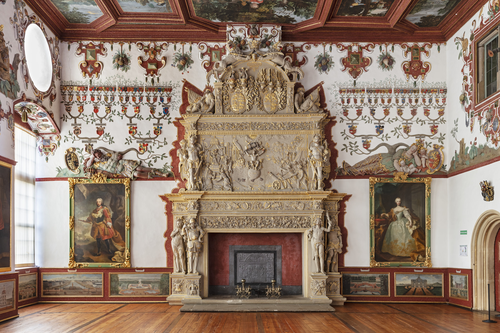
\includegraphics{section_files/figure-pdf/cell-4-output-2.png}
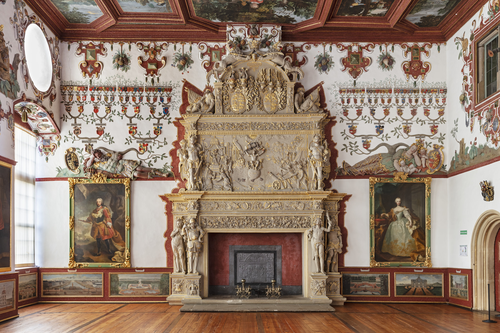
\includegraphics{section_files/figure-pdf/cell-4-output-3.png}

\begin{Shaded}
\begin{Highlighting}[]
\NormalTok{get\_graph()}
\end{Highlighting}
\end{Shaded}

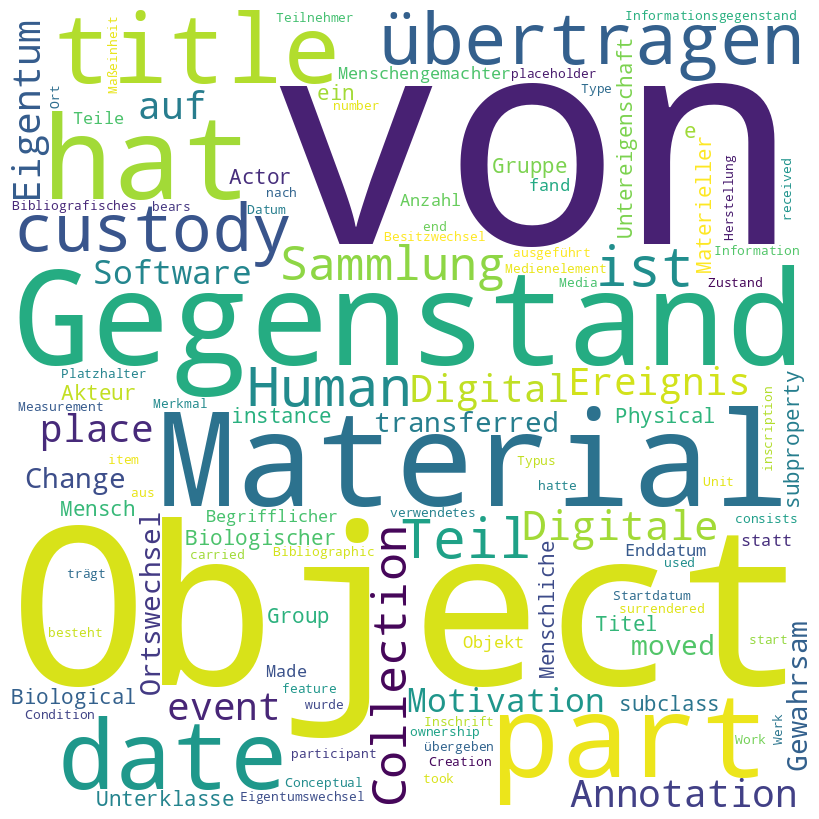
\includegraphics{section_files/figure-pdf/cell-5-output-1.png}


\backmatter

\end{document}
